For the contributions, we had multiple subjects and points within the solution touched on,
which as follow:
\begin{itemize}
    \item Persistence Layer: Which took interest in the implementation of an archival 
        system for the solution, it went in two different ways:
        \begin{itemize}
            \item Implementing the archival for general data that was in JSON format.
            \item Implementing the archival for data that was binary files such as PDFs.
        \end{itemize}
    \item Security Layer: It was the part where we implemented a new filter to the backend,
        specifically for limiting the call backs to the API, through a rate limiter.
        And next was the authentication, which was a migration from a simple Bearer token
        transactional method to a more secure method based on Http Only Cookies storage for
        the token.
    \item Infrastructure: This part mainly targetted, migrating the environment from linux
        virtual machines to managed containers that could offer a better scalability,
        in terms of managing peak load for requests and memory usage.
    \item Continuous integration: Here we implemented a CI/CD pipeline for the solution,
        which took advantage of the previously implemented containerized environment.
        To make the deployment more streamlined and efficient, to allow for easier hot
        fixes and upgrades, and force a better testing of the solution before allowing 
        code to be deployed in an automated fashion.
    \item Refactoring: This was the last point, where the main goal here is to make
        the code more readable and easier to maintain. The trade off is that it will
        take a long time to implement as it requires implementation of a lot of tests
        for the old code. To allow for the beginning of the re-implementation of the
        code, to a newer version that relies on a different architecture.
\end{itemize}

\newpage

\section{Introduction}

So with the context, the problematic and the scope of the project setup, it's 
time to pass to the contributions phase, which consists of conceptual contributions
and their implementation. To be more precise, we'll be handling persistence layer,
security layer, the infrastructure layer and a new deployment strategy.

For each of these layers and phases, we'll be starting with a conceptual or theoretic
study of the solutions we have, and then we'll be talking about the implementation 
projecting it to the project to finally move to the testing and how it was done to validate
the solution used.

\section{Target}\label{sec:target-comp}
As of the current moment the forecast component diagram for the system is as follows:

\begin{center}
    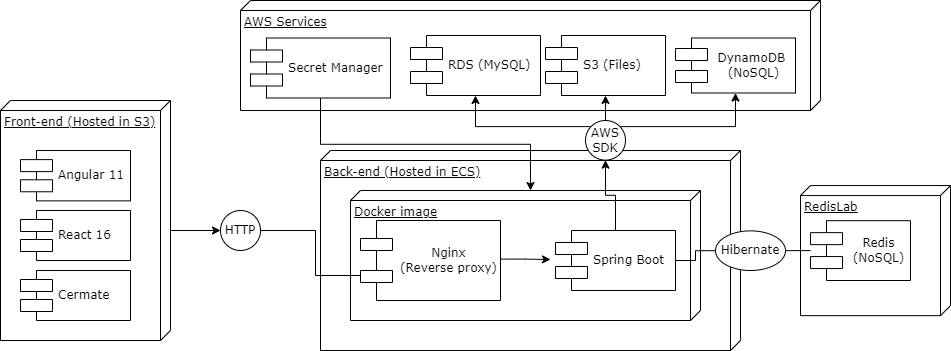
\includegraphics[width=0.8\textwidth]{images/forecast}
\end{center}

As it shows there are additional databases mainly ones for archiving files as is the case of
S3 and also archiving data for statistics down the line thus using DynamoDB\@.
Also containerizing the backend for the goal of having it run different instances seamlessly,
and have the run times duplicate efficiently.
For the creation of the images, it should be noted that they will be generated automatically,
and upload to ECR directly through CircleCI pipelines.
Thus the process of having to update or fix bugs within the back-end will be more streamlined
in a fashion that causes little to no downtime.


\section {Persistence layer}

For the database we had two subjects to study:
\begin{itemize}
        \item Databases for archival purposes
        \item Databases for storing files
    \end{itemize}

\subsection {Archival Database}
So taking the first one, we had to study performance to cost of three solutions and their scalability:

    \begin{itemize}
        \item RDS (SQL)
        \item DynamoDB (NoSQL)
        \item Aurora (SQL)
    \end{itemize}

As all three were AWS solutions, the performance of each was pretty much the same,
and as the database was going to be used for archival it relied less on having a
high throughput and more on how much storage costs.
So we only relied on the cost of the solution, how easy is it to maintain.

So going off by cost first Aurora was the most expensive, with no value added to the problem we'll be solving with it.

So that left us with two options:

    \begin{itemize}
        \item RDS (SQL)
        \item DynamoDB (NoSQL)
    \end{itemize}

We dived into the RDS solution, and it was a bit of a challenge to get it to scale,
in terms of storage compared to DynamoDB which offered autoscaling options and variable
throughput for high load time which could fit the needs of archival as it could take 
higher input in the daily backup process, than the rest of the day.
And for the output there wasn't much to be gained, for neither of the solutions as it was
a rare process that wouldn't be used alot only on demand by the user.

Going to studying the cost, the primary tool that was used for that is the AWS Cost Calculator, which gives rather good indicators to approximate the charges.

\textbf{Case study: }

For the data we used the following:
- 200 Entries per site.
- 500 Site.
- 2 KB per entry.

Site represents the factories and the entries represents the trucks.

So with those inital values, we came to the following results:
- Daily storage of 200 MB or monthly of 6 GB that increments after the period passes.
- 3000000 writes / month
- 100000 reads / month

the reads were just second guessed as there was no significant data about it, 
other than it will be a low read database.

So for the calculations, for RDS we used the following options:
- Instance db.t3.large (vCPU: 2 Memory: 8 GB)
- Instance reserver for one year 
- Single-AZ (1 node)
- 6 GB storage incremented monthly
- 6 GB backup incremented monthly

which resulted in the yearly cost of \$1185.769

For DynamoDB, we used the following options:
- Standard-Infrequent Access (Reduces cost of storage)
- 3 Mil writes per month
- 100K reads per month
- 6 GB storage incremented monthly
- 6 GB backup incremented monthly

Which came down to the cost of \$236.00 per year.

As we can notice the RDS cost was much higher than DynamoDB,
so we decided to use DynamoDB as it was cheaper, and also had
better maintenance options offered by AWS as it's a fully hosted
service.

Lastly, the only missing part was integration within the back-end which went on different steps.

First we had to create a service on the Spring Back-end that took on the handling of the communication layer between the DB and the back taking on mulitple functionalities such as:

    \begin{itemize}
        \item Creating - delete tables
        \item Creating indexes to allow fast access to the data
        \item Adding - deletting data
        \item Finding data using specific fields
    \end{itemize}

Then implementation of unit tests for the service to ensure that it's working as intended,
it had taken on the following tests:

    \begin{itemize}
        \item Create table for tests with required indexes
        \item Adding data to table, and then finding it
        \item Adding data to table, and find it by date
        \item Adding data to table, and find it by different keys
        \item Cleaning up the table
    \end{itemize}

The creation of the tables and their indexes was automated, to allow for the
reproduction of the same environment for the data we had during testing, and in the 
dev environment. Also, getting rid of the need for manual creation of the tables.

\begin{figure}[!htb]
    \centering
    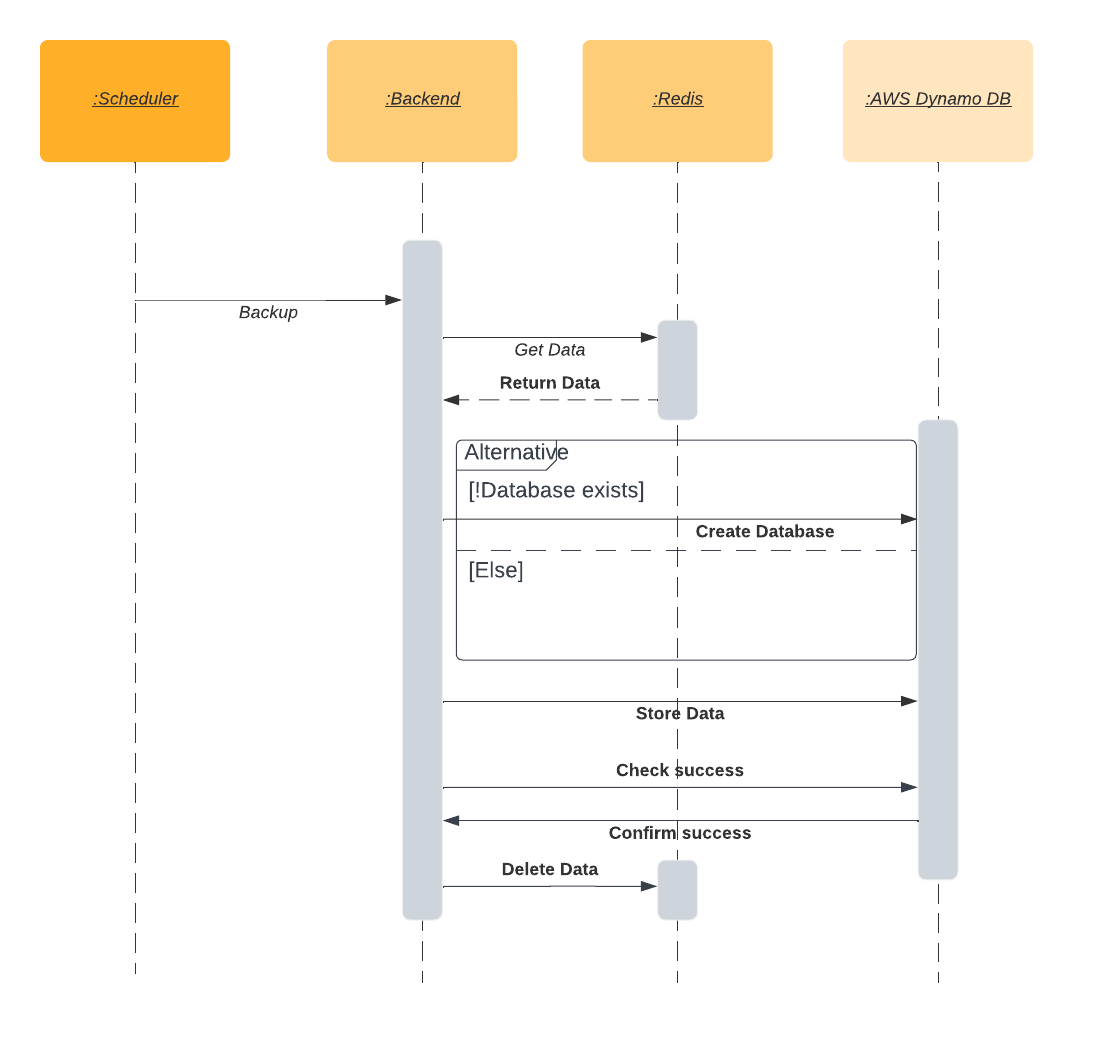
\includegraphics[width=0.8\textwidth]{images/archival_backup.png} 
    \caption{\footnotesize{Archival Cronjob}}
    \label{fig:archival_backup}
\end{figure}

Finally the archival process came as a cronjob shown in figure \ref{fig:archival_backup},
that would take the data each day at 00:00 and archive it from the redis database to the
DynamoDB while checking that everything was successfully archived before cleaning the data
from Redis.



\subsection {File storage Database}
For this second database, that is more opted to be used for the storage of files.
The solution was already known, and was the Amazon S3 service.

The file storage database was used for the following:

    \begin{itemize}
        \item Storing site configuration files
        \item Storing client files
    \end{itemize}

The storage was pretty simple, it was just a bucket with a specific folder structure.
So for the first case it was a folder for each site,
and for the second it was a folder for each client which was handled with the archival
cronjob as these files were related to the data from the trucks that have been handled
during the day.

For the tests we used the following:

    \begin{itemize}
        \item Creating a bucket
        \item Creating a folder structure
        \item Adding data to the bucket and finding it
        \item Deleting data from the bucket
        \item Deleting the bucket
    \end{itemize}

For the creation of the bucket it was made such as it's done automatically once the
server started in case it doesn't exist.
So that we can reproduce the same bucket that there was in the dev environment and during
the  tests.


\section {Security and Authentication}

\subsection {Ratelimiting} \label{subsec:ratelimiting}
rate limiting was one interesting aspect for security, as it's a way to prevent the
server from being flooded with requests. As it could stop DDOS attacks, brute force
attacks, and any other kind of attack that would require sending lot of request from 
the same IP or same user.

For the rate limiting, as we were using already a Spring backend we had a couple options
to choose from the first one was Bucket4j, which is a rate limiter that relies on token
bucket algorithm which approaches rate limiting through putting a number of tokens in a
bucket then whenever the consume or client tries to use a service it has to consume one
or more tokens from the bucket until they are depleted then the client is blocked,
the bucket is then assigned to a key which could be a user, IP address or API key ...

The second option was to use Resilience4j, which relies on creating cycles where each cycle
has a number of allowed permissions and refreshes in the beginning of each cycle, which
allows the handling of the rate limiting in a epoch fashio but it was not easy to
implement for the case of a distributed backend and not worth the trouble to adapt it
with a caching system within the Redis Database to do so, as it relied heavily on
single machines threads for the handling it does.

So we went with the former, which was implemented as a filter within the API gateway
in the Spring backend as shown figure \ref{fig:b4j}.

\begin{figure}[!htpb]
    \centering
    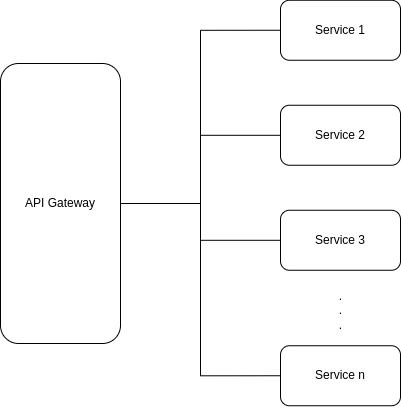
\includegraphics[width=0.5\textwidth]{images/ratelimiting.png}
    \caption{\footnotesize{Backend Gateway}}
    \label{fig:b4j}
\end{figure}


So the now the handling of services within the Java Spring backend required the passage
from API rate limiter which consisted of giving a token to the client before allowing
the request to be processed, and this requests were by default capped to a certain number
that could be modified through the configuration file of the server.

Now with the basic handling in hand, we opt for the implementation of the rate limiter
which was done in two ways, the first was to have a bucket for each user,
and the second was to have a bucket for each IP address.

Rate limiting the user was specifically setup for handling the private endpoints and that
was able to be modified by the admin to allow for more or less requests per second
depending on the user, and the rate limiting the IP address was setup for the public API.

And lastly there was the rate limiting for the login, which was individually handled for
the purpose of limiting the number of login attempts per minute to avoid possibility
of a dictionnary attacks.



\subsection {Authentication}
The authentication was also one of the interesting aspects for security, as it's a way to
prevent confidential data from being accessed without having the right credentials. But the 
prior used solution was having a permanent JWT token that is acquired during the login, meaning 
that once the that Token is generated it could be permanently used to access the data as it didn't
use any additional timing parameter to expire the token.

As for that, came the need to implement a ephemeral token, which is a token that gets expired after
a certain time, to access the data and opted to add a refreshing mechanism which was to make the
user experience better to avoid the need of having them reconnect within their sessions.

But not only that, we also opted to move from a Bearer token transportation of the token to a HTTP Only cookie,
which is a cookie that is only accessible through the HTTP protocol, not the Javascript and is proclaimed to
be the safest option to store the JWT. And then proceeded to embed the token within the cookie,
as so we can avoid the possiblity of exploitation through JS injections to acquire the token.

The authentication had a simple flow \ref{fig:token}, the user presented his credentials,
the server validated them, in case they were valid the server would generate a new access 
token, which was embedded in the header as a HTTP Only cookie then that would make 
all the request coming from the front end to the server to have the token in the header
with no need for the Javascript to do any handling for that last.

\begin{figure}[!htbp]
    \centering
    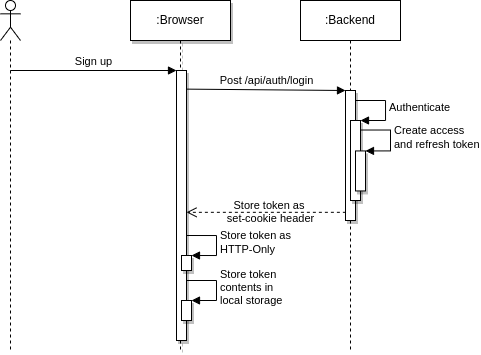
\includegraphics[width=0.75\textwidth]{images/JWTHttpOnly.png}
    \caption{\footnotesize{JWT HTTP Only Cookie}}
    \label{fig:token}
\end{figure}

The refresh token mechanism was to make the user experience better and also to increase
the security of the application, make the intercepted JWT tokens mostly come in useless
if they were caught late, as they would be expired.

So the flow \ref{fig:refresh} of that was to that during the login there was a generation
of access token and refresh token, the referesh token came in handy to create a new access
token once the old one has expired and the user was still active during that session, to
avoid forcing the user to re-login.

\begin{figure}[!htbp]
    \centering
    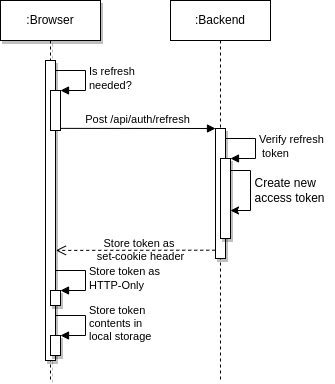
\includegraphics[width=0.42\textwidth]{images/refresh.png}
    \caption{\footnotesize{Refresh token}}
    \label{fig:refresh}
\end{figure}

\newpage


\section {Containerization and Deployment}
Before we dive in into the specifics, we first will showcase the final architecture in the
Elastic Container Service (ECS), which is a fully managed container orchestration service,
more information about the ECS can be found in the following link \cite{ecs_intro}

\begin{figure}[!ht]
    \centering
    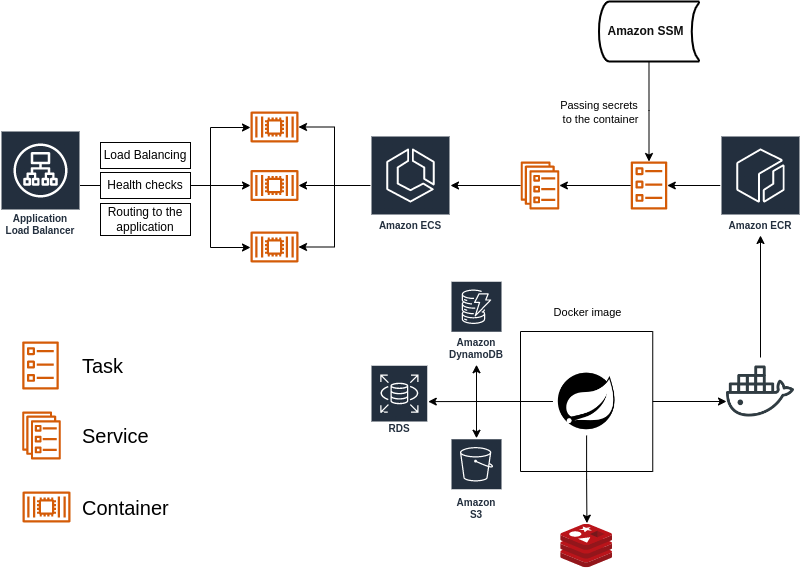
\includegraphics[width=\textwidth]{images/ECS}
    \caption{\footnotesize{ECS Architecture}}
    \label{fig:ECSArch}
\end{figure}

Task: the component which takes care of running the containers.

Service: the component which manages the tasks.

Container: the image that is running on the task.

\subsection {ECS Containerization and secrets}

The ECS solution shown in figure \ref{fig:ECSArch} was a bit of a challenge to get it to
work, as it was a containerized solution, and not a native one.
So the first step was to containerize the solution, and have a safe image that doesn't
expose any secrets or environment variables.

In the docker way, we can just pass them through the command line,
and the solution will run perfectly.

But here relied a problem that was the ECS solution, it didn't have a simple
way to feed it the credentials, environment variables neither files, so we had to opt
for using the SSM or Secrets Manager
which is yet another hosted solution to store strings as secrets, and then those could be 
passed to the ECS services.

With the Secrets Manager, for the strings secrets it was a simple writing / reading process
to store and retrieve the secrets. But for the files it was a bit more complicated, there
wasn't a direct way to do that.

Finally we came up with the following solution, which is as follows:

\begin{itemize}
    \item Serialize the content of the file into a base64 string
    \item Store the base64 string in the AWS Systems Manager (SSM)
    \item Pass the SSM secret to the ECS service
    \item Retrieve the secret from the SSM as a environment variable
    \item Decode the base64 string
    \item Store the deserialized base64 in a file in the container
    \item Point an environment variable to the file
\end{itemize}

As such we managed to pass aws credentials, google credentials and Redis Labs credentials.

\subsection {Load Balancer and routing}

As shown in the ECS Architecture, we had a load balancer in front of the running tasks, which has four main goals:

\begin{itemize}
    \item To take care of the incoming traffic from the client side
    \item To ensure that the traffic distributed evenly
    \item To ensure that the tasks are healthy
    \item To ensure that the tasks are not overloaded and manage it's scalability.
\end{itemize}

\begin{figure}[!htbp]
    \centering
    \includegraphics[width=\textwidth]{images/loadBalancer.png}
    \caption{\footnotesize{Load Balancer Interaction with the backend}}
    \label{fig:loadbalancer}
\end{figure}

So the load balancer is as shown in figure \ref{fig:loadbalancer}, it took traffic from
port 80 where it had an exposed dns link, then it routed it through a VPS to the
containers that are exposing post 8080 in their local network, having healthchecks
done on the endpoint /actuator/health .

With that set in place, we had pretty much everything setup to start testing for the
load handling by the ecs to check for the health of the containers and the measures
to be set to ensure that the auto scaling is setup with the right parameters.

So first, we written scripts that did kind of overload the server with the requests,
asynchronously deploy the containers and check monitoring metrics.

\begin{figure}[!ht]
    \centering
    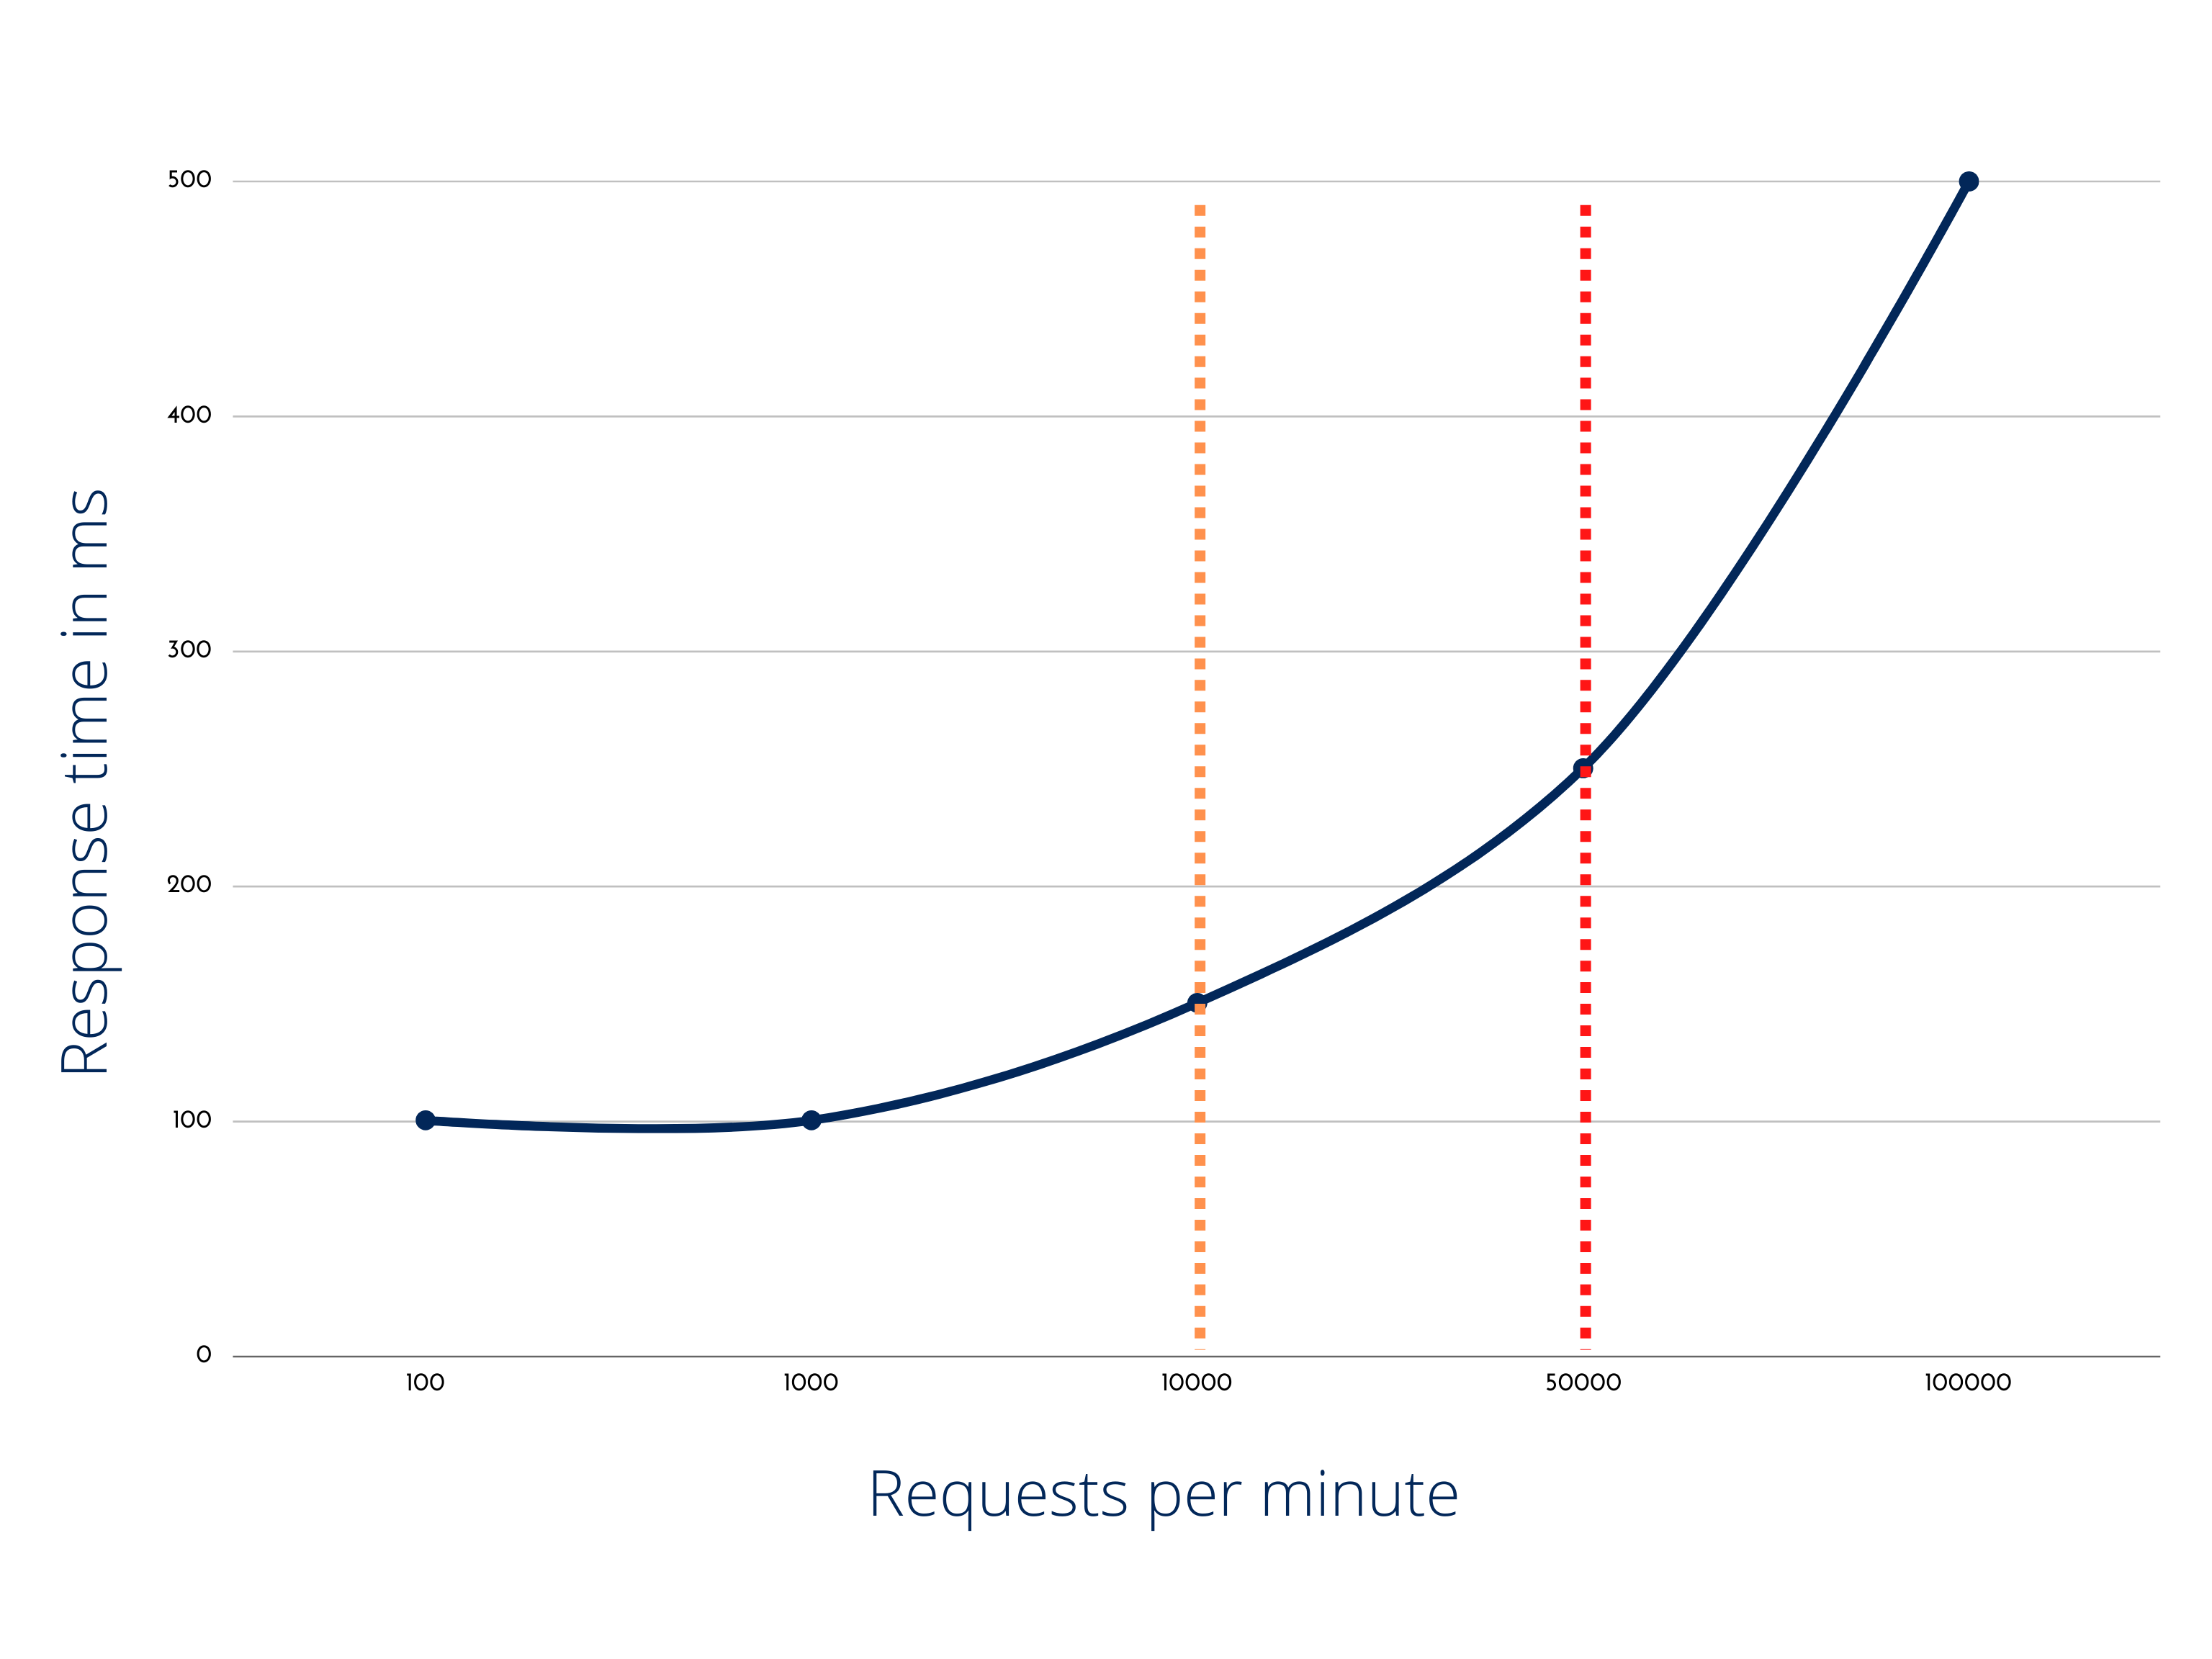
\includegraphics[width=\textwidth]{images/assesment_autoscaling.png}
    \caption{\footnotesize{Auto Scaling Assessment}}
    \label{fig:autoscaling_assessment}
\end{figure}

So next came doing the assessment of autoscaling, we ended up compiling the chart
in figure \ref{fig:autoscaling_assessment} which shows the response time per
number of requests sent per minute, the assesment was done by using a script
written in Scala.
Looking at the chart we can see that the response time was pretty stable until
we reached the 10000 requests mark, where there was a clear increase but nothing
that could kill the usage till we exceeded the 50000 mark where the response time
was getting really high meaning that at this point there's no advantage on keeping
only the existing instances up but the need to increase becomes apparent, and that
was due to the heavy requests creating a sort of queue in the backend which would
require multiple processes thus comes the horizontal increase advantage in the ECS.

So firstly, as shown in \ref{fig:loadtest} it took the endpoint to be hit, in case
it was a private endpoint you'd need to provide the credentials to. Then put in place
the number of requests to be sent and finally run it.

Once it started running it was a simple case of sending requests asynchronously in fibers
or virtual threads, and then printing the response time of each request, as such we could
monitor the handling time of the requests being affected by the load of requests.

\begin{figure}[!ht]
    \centering
    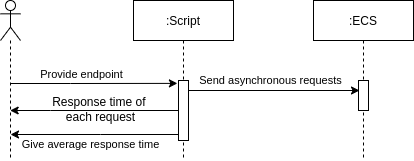
\includegraphics[width=0.8\textwidth]{images/scriptdos.png}
    \caption{\footnotesize{Load Test Script}}
    \label{fig:loadtest}
\end{figure}


Thus it we could find the right parameters for the autoscaling, based on the number of
requests being sent per minute, which at the time of tests was around 50000 requests per
minute without the response time being affected which is quite impressive.

And as most the back-end services relying heavily on the memory, we ensured to put a 70\%
memory usage limit on the containers before spawning new instances to handle the load, in
case of autoscaling by memory.

Next came the assesment and benchmarking of two databases solutions which were a Redis
instance hosted in EC2, and a Redislabs hosted instance.

The tests were done by using a script that was written in python, and it was a
stress testing script, which sole purpose was to overload the Redis instance 
and then check if the requests then took longer to fulfill, as Redis was a in-memory
database, so the goal of using it was speed.

\begin{table}[!ht]
    \centering
    \begin{tabular}{| c | c |}
        \hline
        \textbf{Database} & \textbf{Stress Test} \\
        \hline
        Redis on EC2 & 
                \begin{tabular}{| c | c |}
                    \textbf{Load} & \textbf{Response by Endpoint} \\
                    \hline
                    \textbf{25\%} &
                            \begin{tabular}{| c | c |}
                                \textbf{Endpoint} & \textbf{Response Time} \\
                                \hline
                                Add client & \textbf{129.9} \\
                                \hline
                                Get all clients & \textbf{89.9} \\
                                \hline
                                Heavy Load Enpoint & \textbf{269.2} \\
                            \end{tabular}\\
                    \hline
                    \textbf{50\%} &
                            \begin{tabular}{| c | c |}
                                \textbf{Endpoint} & \textbf{Response Time} \\
                                \hline
                                Add client & \textbf{128.3} \\
                                \hline
                                Get all clients & \textbf{106.1} \\
                                \hline
                                Heavy Load Enpoint & \textbf{245.7} \\
                            \end{tabular}\\
                    \hline
                    \textbf{75\%} &
                            \begin{tabular}{| c | c |}
                                \textbf{Endpoint} & \textbf{Response Time} \\
                                \hline
                                Add client & \textbf{133.6} \\
                                \hline
                                Get all clients & \textbf{196.1} \\
                                \hline
                                Heavy Load Enpoint & \textbf{257.7} \\
                                \hline
                            \end{tabular}\\
                \end{tabular}\\
        \hline
        Redis on RedisLab & 
                \begin{tabular}{| c | c |}
                    \textbf{Load} & \textbf{Response by Endpoint} \\
                    \hline
                    \textbf{25\%} &
                            \begin{tabular}{| c | c |}
                                \textbf{Endpoint} & \textbf{Response Time} \\
                                \hline
                                Add client & \textbf{154.1} \\
                                \hline
                                Get all clients & \textbf{79.5} \\
                                \hline
                                Heavy Load Enpoint & \textbf{256.8} \\
                            \end{tabular}\\
                    \hline
                    \textbf{50\%} &
                            \begin{tabular}{| c | c |}
                                \textbf{Endpoint} & \textbf{Response Time} \\
                                \hline
                                Add client & \textbf{134.1} \\
                                \hline
                                Get all clients & \textbf{126.4} \\
                                \hline
                                Heavy Load Enpoint & \textbf{241.2} \\
                            \end{tabular}\\
                    \hline
                    \textbf{75\%} &
                            \begin{tabular}{| c | c |}
                                \textbf{Endpoint} & \textbf{Response Time} \\
                                \hline
                                Add client & \textbf{143.5} \\
                                \hline
                                Get all clients & \textbf{156.3} \\
                                \hline
                                Heavy Load Enpoint & \textbf{258.2} \\
                                \hline
                            \end{tabular}\\
                \end{tabular}\\
        \hline
    \end{tabular}
    \caption{\footnotesize{Stress testing Redis against RedisLab}}
    \label{tab:stress_testing}
\end{table}

The results on the table above were quite impressive, as the response time of the
requests was quite low, and the load was quite high, the only noticeable growth was
in the response time of the Get All Clients and that was due to the fact that to 
increase the load on the Redis instance we had to increase the number of clients.
Thus, get all clients got heavier and heavier to handle.

As shown in \ref{tab:stress_testing}, it ended up being with a pretty close result,
no one over ruling the other, and the results were pretty close to the expected results.
So we ended up either having to opt for the Redis instance hosted in EC2 and do 
all the configuration manually which would lead to a lot of configuration done manually,
or just resorting to the Redislabs hosted instance, as it's a fully managed instance.
All the security measures and replication are taken care of by cloud host.

\subsection{Deployment}

Finally after testing everything, and having deployed one ECS service succesfully, we had
to automate the deployment process, so that we could handle new versions and code update
without much effort.

This came in the form of a gradle task, which was as follows:

    \begin{figure}[!htbp]
        \centering
        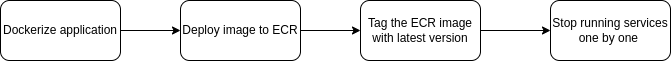
\includegraphics[width=\textwidth]{images/gradle.png}
        \caption{\footnotesize{Deployment of the App to ECS - Gradle Task}}
        \label{fig:gradle}
    \end{figure}

The dockerization part of the gradle task was handled using a third party plugin,
then the deployment to Elastic Container Registry (ECR\footnote{ECR is an AWS managed
    container image registry service that is secure, scalable, and reliable. More
    information can be found in \cite{ecr_intro}.})e using the AWS CLI,
by linking the ECR to docker, then pushing the image is automatically uploaded to ECR.
Once this is done, the ECS service has to handle the update of the image, 
and this was done through a bash script that took in charge of getting a list 
of the running tasks, then stopping one of them, and wait for a new one to spawn 
such as to avoid down time during the update of the service.

    \begin{figure}[!ht]
        \centering
        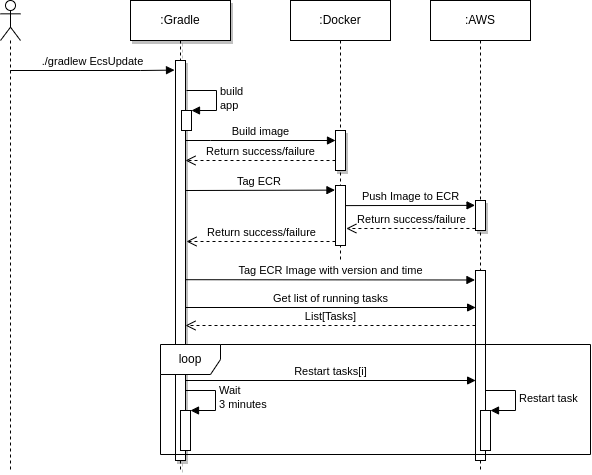
\includegraphics[width=0.9\textwidth]{images/gradleTask.png}
        \caption{\footnotesize{Deployment Sequence Diagram}}
        \label{fig:deployment}
    \end{figure}

So in the figure \ref{fig:deployment}, the flow is pretty simple,
it goes as follows:

    \begin{itemize}
        \item Gradle builds the docker image using a 3rd party plugin
        \item Tag image with right version of the application and push it to ECR
        \item Tag ECR image with current version in addition to timestamp it
        \item Get the list of running tasks
        \item Stop one of the running tasks
        \item Wait for a new one to spawn
        \item The two last steps are repeated till the list is exhausted
    \end{itemize}

And in such a way, we can handle the deployment without having any downtime,
so it makes introducing bug fixes a better experience for both developer and 
customer.



\section {Continuous Integration}
\subsection{What is continuous integration?}

Continuous integration(CI) is a technique for building software incrementally, as in a way
to automate the build and testing of the code. This method encourages developers to 
write code that is more readable, more maintainable, and more testable. Also it makes
it easier to find bugs before they are introducted into the main code, and to
catch as much problems as possible before the code reaches the production environment.

CI has emerged as a great tool for software development, as it eases the process of
merging code from different branches which allows for a more efficient development process,
as developers mostly work on their own branch in isolation, and this allows them to 
introduce features and fixes that integrate with the rest of the code. \cite{ci_msft}

Along with CI, there is Continuous Delivery(CD), which is the other end of this process
and is used to push code to a production environment, allowing for smoother introduction
of updates, hotfixes, \dots

\subsection{CI/CD projected on the system}

As one of the most important features within the industrialization of the project
was having a reliable and maintainable deployment process, here where came the 
continuous intagration pipelines. The CI pipeline offered a great way to have
a reliable and maintainable deployment process and to automate the whole process
of the project.

\begin{figure}[!htpb]
    \centering
    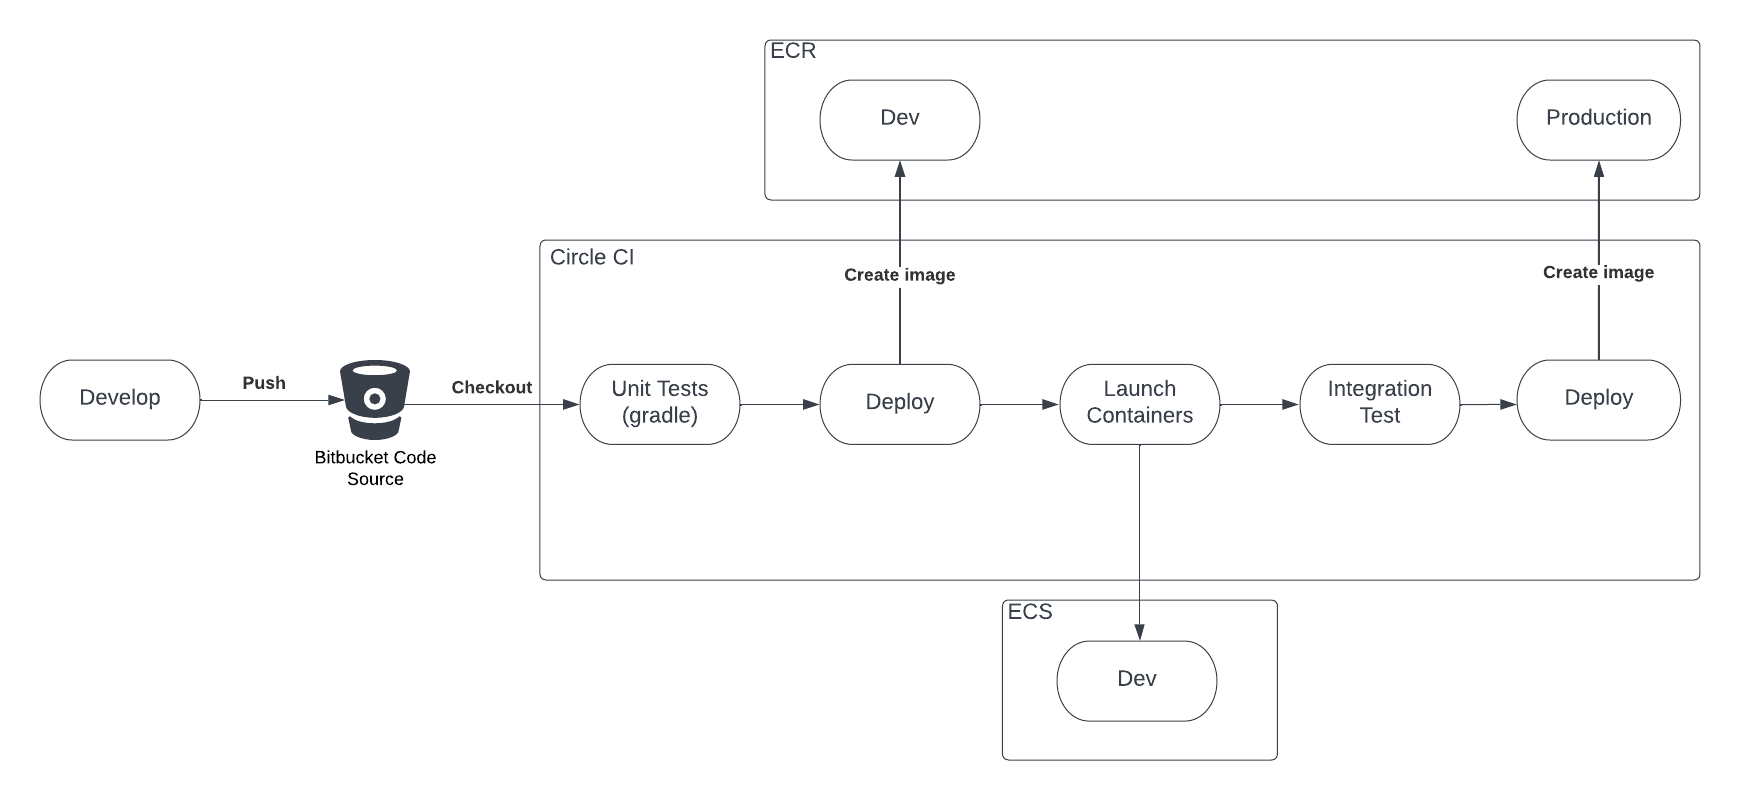
\includegraphics[width=\textwidth]{images/ci-cd-pipeline.png}
    \caption{Continuous integration pipeline}
    \label{fig:ci-cd-pipeline}
\end{figure}

As shown in the figure \ref{fig:ci-cd-pipeline}, the CI pipeline is composed
of three main steps:
    \begin{itemize}
        \item \textbf{Test}: the test phase is the first step of the CI pipeline.
            It is responsible for running the tests built on the project using
            the gradle test task.
        \item \textbf{Coverage}: the coverage phase is the second step of the CI pipeline.
            It uses SonarScanner, which is a scanner for code analytics reporting things
            from code quality to security threats. It generates the coverage report of the
            project and then it sends the report to the SonarCloud\footnote{SonarCloud is
                a cloud service used for hosting SonarQube scans} server.
        \item \textbf{Build and Deploy}: the build and deploy phase is the last step
            of the CI pipeline. It is responsible for building a docker image and then
            pushing it to ECR (EC Container Registry) and then deployed to ECS
            (ECS Container Service) all that using a range of custom scripts built
            by us within gradle, to ease up the deployment within the pipeline.
    \end{itemize}

The CI/CD service we've went for was the Circle CI, which is a hosted continuous
integration service that is used to test the code and to deploy the application.
The configuration of the CI/CD service was configured within a yaml file,
which is located in the \texttt{.circleci/config.yml} file.

The test and building steps both came from taking advantage of the gradle build
system, which were already setup and configured within the project. But nonetheless,
as the CI/CD pipeline creates docker containers to run the tests and the build,
and the tests needed AWS credentials to be able to run, we had to somehow pass
the file containing the AWS credentials to the CI/CD pipeline, which was done
by creating new AWS credentials creating a AWS credentials file then encoding to
base64 and passing it to the CI/CD pipeline as a environment variable, then decoding
it to a string to be stored in the \texttt{.aws/credentials} inside the pipeline which
was a play around to pass the files to any virtualized environment not allowing for 
those accesses.

Next came the coverage phase, which was a bit more involved. The coverage takes care
of analyzing the code to see if there are any security issues, bugs, bad code and
everything that relate to code analysis, and then it sends the report to the
SonarCloud server. The important thing in this phase is that it can be as a test to
the code's quality, so you can set the threshold of the coverage to be a certain
percentage, and if the coverage is below that threshold, then the CI/CD pipeline
will fail so we can stop critical issues from being deployed if they weren't caught
during development.

The deployment, which is the last step of the CI pipeline, is done using orbs
within Circle CI, orbs are snippets of codes used to automate repeatable processes
and published by the Circle CI team, specifically the ECR and ECS orbs.

As the orbs didn't come in handy, as we had different way of building the docker image
than the default one, we opted to creating our own job within the CI/CD pipeline
which took care of the building and deployment phase of the project.
The job went as follow: 
    \begin{itemize}
        \item Create a docker image using the gradle build tool.
        \item Tag the docker image with the project name.
        \item Push the docker image to ECR.
        \item Set ECR image with the right tags.
        \item Restart the ECS running tasks to run the new image.
    \end{itemize}

In the end, the CI/CD pipeline was configured to only build and deploy on two branches
which are "master" to deploy on the production environment and "dev" to deploy on the
development environment.


\section {Refactoring and Improvements}\label{sec:refactoring}
\subsection {Adding user management system}

The old system didn't have a user management system, as it relied on the site being the
user so there wasn't really users to manage. So we had to integrate users within the system
then add a way to manage them, and this was done by migrating the site from being the user
to being an entity that could be managed by users who have the right to do so.
And that required rework through the majority of the backend as this architecture was
relied on by all the backend services and controller and also frontend.

So we had to change this architecture to be able to manage users and their roles, but also
keep the old behaviour the same.

%TODO: Add class diagram before and after (Couldn't do it now because we migrated directly without using diagrams)

\subsection {Implementation of tests for existing codebase}

TODO: Still not touched on yet


\section {Conclusion}

To conclude, during the implementation of the subjects, we had implemented a lot of
new features and improvements ranging from databases and security, to infrastructure 
and deployment.
As we've seen during the last section \ref{sec:refactoring}, the refactoring wasn't 
implemented yet, but the main goal of this phase has been discussed in such a way
that it will be easier to implement the refactoring in the future.
The main goal of this contributions phase was to make the ground work for a more rigid
and upgradable solution, which would allow for the development of a more robust and
upgradable solution once the refactoring is fully implemented.

